% ============================================================
% Chapitre 1 : Statistique Descriptive
% ============================================================
\chapter{Statistique Descriptive --- R\'esum\'e et Visualisation}
\label{ch:descriptive}

\begin{center}
\textit{<<~On ne peut am\'eliorer que ce que l'on mesure.~>>} --- Lord Kelvin
\end{center}

% ------------------------------------------------------------
\section{Exemple motivant}
% ------------------------------------------------------------

Une entreprise poss\`ede les salaires mensuels (en euros) de ses 20 employ\'es :
\[
1800,\; 1950,\; 2100,\; 2100,\; 2200,\; 2300,\; 2350,\; 2400,\; 2500,\; 2600,
\]
\[
2650,\; 2700,\; 2800,\; 2900,\; 3100,\; 3200,\; 3500,\; 3800,\; 4500,\; 8000.
\]
Questions naturelles : quel est le salaire <<~typique~>> ? Les salaires sont-ils dispers\'es ? Y a-t-il des valeurs aberrantes ? Pour y r\'epondre, il faut \emph{r\'esumer} et \emph{visualiser} les donn\'ees.

% ------------------------------------------------------------
\section{Population, \'echantillon, variables}
% ------------------------------------------------------------

\begin{definition}[Population et \'echantillon]
\index{population}\index{echantillon@\'echantillon}
La \textbf{population} est l'ensemble complet des individus \'etudi\'es. Un \textbf{\'echantillon} de taille $n$ est un sous-ensemble $(x_1,\ldots,x_n)$ de la population.
\end{definition}

\begin{definition}[Types de variables]
\index{variable!qualitative}\index{variable!quantitative}
\begin{itemize}
\item \textbf{Variable qualitative} (cat\'egorielle) : valeurs dans un ensemble fini de cat\'egories.
  \begin{itemize}
  \item \emph{Nominale} : pas d'ordre naturel (couleur, sexe).
  \item \emph{Ordinale} : ordre naturel (mention au bac : passable $<$ AB $<$ B $<$ TB).
  \end{itemize}
\item \textbf{Variable quantitative} : valeurs num\'eriques.
  \begin{itemize}
  \item \emph{Discr\`ete} : valeurs dans un ensemble d\'enombrable ($\N$, nombre d'enfants).
  \item \emph{Continue} : valeurs dans un intervalle de $\R$ (taille, poids).
  \end{itemize}
\end{itemize}
\end{definition}

% ------------------------------------------------------------
\section{Mesures de tendance centrale}
% ------------------------------------------------------------

\begin{definition}[Moyenne arithm\'etique]
\index{moyenne}
Pour un \'echantillon $(x_1,\ldots,x_n)$, la \textbf{moyenne} est :
\[
\bar{x} = \frac{1}{n}\sum_{i=1}^{n} x_i.
\]
\end{definition}

\begin{definition}[M\'ediane]
\index{mediane@m\'ediane}
La \textbf{m\'ediane} $\mathrm{Me}$ est la valeur qui s\'epare l'\'echantillon ordonn\'e en deux moiti\'es \'egales. Si $x_{(1)}\leq x_{(2)}\leq\cdots\leq x_{(n)}$ d\'esigne l'\'echantillon ordonn\'e :
\[
\mathrm{Me} = \begin{cases}
x_{((n+1)/2)} & \text{si } n \text{ est impair,}\\
\frac{1}{2}\left(x_{(n/2)}+x_{(n/2+1)}\right) & \text{si } n \text{ est pair.}
\end{cases}
\]
\end{definition}

\begin{definition}[Mode]
\index{mode}
Le \textbf{mode} est la valeur la plus fr\'equente de l'\'echantillon.
\end{definition}

\begin{intuition}
La moyenne est sensible aux valeurs extr\^emes ; la m\'ediane est \textbf{robuste}. Dans l'exemple des salaires, $\bar{x}=3007{,}50$~\texteuro{} est tir\'ee vers le haut par le salaire de 8000~\texteuro{}, tandis que $\mathrm{Me}=2625$~\texteuro{} refl\`ete mieux le salaire <<~typique~>>.
\end{intuition}

% ------------------------------------------------------------
\section{Mesures de dispersion}
% ------------------------------------------------------------

\begin{definition}[Variance et \'ecart-type]
\index{variance}\index{ecart-type@\'ecart-type}
La \textbf{variance empirique} (corrig\'ee) et l'\textbf{\'ecart-type} sont :
\[
s^2 = \frac{1}{n-1}\sum_{i=1}^{n}(x_i-\bar{x})^2, \qquad s = \sqrt{s^2}.
\]
La version non corrig\'ee utilise $n$ au d\'enominateur. Le facteur $n-1$ (correction de Bessel) garantit que $s^2$ est un estimateur sans biais de la variance de la population (cf.\ chapitre~\ref{ch:proprietes}).
\end{definition}

\begin{definition}[\'Etendue et \'ecart interquartile]
\index{etendue@\'etendue}\index{ecart interquartile@\'ecart interquartile}
\begin{align}
\text{\'Etendue} &= x_{(n)} - x_{(1)}, \\
\text{IQR} &= Q_3 - Q_1,
\end{align}
o\`u $Q_1$ et $Q_3$ sont les premier et troisi\`eme quartiles (m\'edianes des moiti\'es inf\'erieure et sup\'erieure).
\end{definition}

\begin{definition}[Coefficient de variation]
\index{coefficient de variation}
Le \textbf{coefficient de variation} est le rapport $\mathrm{CV} = s/\bar{x}$ (pour $\bar{x}\neq 0$). Il permet de comparer la dispersion de variables d'unit\'es diff\'erentes.
\end{definition}

% ------------------------------------------------------------
\section{Mesures de forme}
% ------------------------------------------------------------

\begin{definition}[Coefficient d'asym\'etrie (skewness)]
\index{asymetrie@asym\'etrie}\index{skewness}
\[
\gamma_1 = \frac{1}{n}\sum_{i=1}^n\left(\frac{x_i-\bar{x}}{s}\right)^3.
\]
$\gamma_1>0$ : queue \`a droite (asym\'etrie positive). $\gamma_1<0$ : queue \`a gauche. $\gamma_1=0$ : distribution sym\'etrique.
\end{definition}

\begin{definition}[Coefficient d'aplatissement (kurtosis)]
\index{kurtosis}\index{aplatissement}
\[
\gamma_2 = \frac{1}{n}\sum_{i=1}^n\left(\frac{x_i-\bar{x}}{s}\right)^4 - 3.
\]
$\gamma_2=0$ pour une distribution normale (mesosurtique). $\gamma_2>0$ : queues lourdes (leptokurtique). $\gamma_2<0$ : queues l\'eg\`eres (platykurtique).
\end{definition}

% ------------------------------------------------------------
\section{Repr\'esentations graphiques}
% ------------------------------------------------------------

\subsection{Histogramme}
\index{histogramme}

L'histogramme repr\'esente la distribution d'une variable quantitative continue en regroupant les valeurs en classes.

\begin{center}
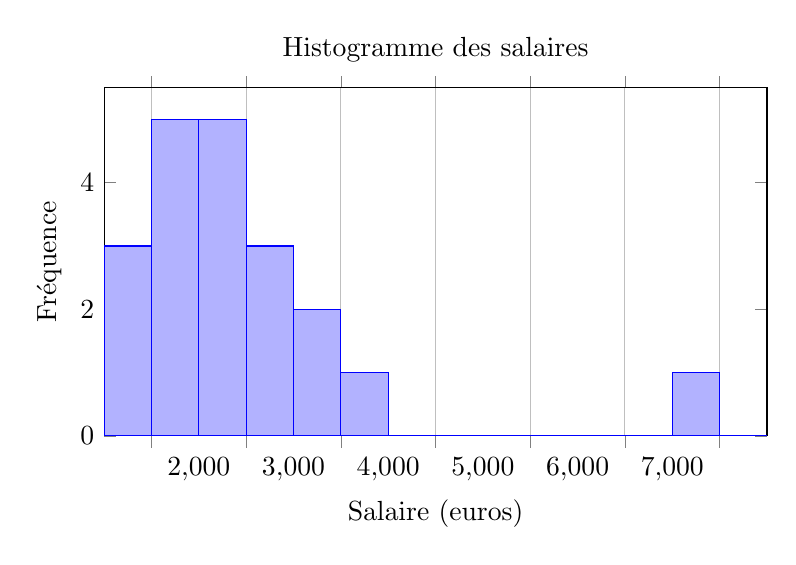
\begin{tikzpicture}
\begin{axis}[
    ybar interval,
    width=10cm, height=6cm,
    xlabel={Salaire (euros)},
    ylabel={Fr\'equence},
    xmin=1500, xmax=8500,
    ymin=0,
    xtick={2000,3000,4000,5000,6000,7000,8000},
    title={Histogramme des salaires}
]
\addplot coordinates {
    (1500,3) (2000,5) (2500,5) (3000,3) (3500,2) (4000,1) (4500,0) (5000,0) (5500,0) (6000,0) (6500,0) (7000,0) (7500,1) (8000,0) (8500,0)
};
\end{axis}
\end{tikzpicture}
\end{center}

\subsection{Bo\^ite \`a moustaches (boxplot)}
\index{boite a moustaches@bo\^ite \`a moustaches}

\begin{center}
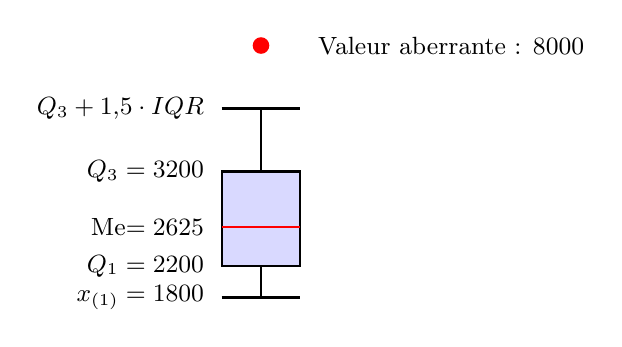
\begin{tikzpicture}
  % Boxplot manuel
  \draw[thick] (2,0) -- (2,0.4);       % min whisker
  \draw[thick] (1.5,0) -- (2.5,0);     % min bar
  \draw[thick,fill=blue!15] (1.5,0.4) rectangle (2.5,1.6); % boite
  \draw[thick,red] (1.5,0.9) -- (2.5,0.9); % mediane
  \draw[thick] (2,1.6) -- (2,2.4);     % max whisker
  \draw[thick] (1.5,2.4) -- (2.5,2.4); % max bar
  \fill[red] (2,3.2) circle (3pt);     % outlier
  % labels
  \node[left] at (1.4,0) {\small $x_{(1)}=1800$};
  \node[left] at (1.4,0.4) {\small $Q_1=2200$};
  \node[left] at (1.4,0.9) {\small Me$=2625$};
  \node[left] at (1.4,1.6) {\small $Q_3=3200$};
  \node[left] at (1.4,2.4) {\small $Q_3+1{,}5\cdot\text{IQR}$};
  \node[right] at (2.6,3.2) {\small Valeur aberrante : $8000$};
\end{tikzpicture}
\end{center}

\subsection{Diagramme en b\^atons et diagramme circulaire}

Le diagramme en b\^atons convient aux variables discr\`etes ; le diagramme circulaire (camembert) aux variables qualitatives nominales avec peu de modalit\'es.

\subsection{Fonction de r\'epartition empirique}
\index{fonction de repartition empirique@fonction de r\'epartition empirique}

\begin{definition}
La \textbf{fonction de r\'epartition empirique} est :
\[
\hat{F}_n(x) = \frac{1}{n}\sum_{i=1}^n \mathbf{1}_{x_i \leq x}.
\]
C'est une fonction en escalier qui approche la vraie fonction de r\'epartition $F$ (th\'eor\`eme de Glivenko--Cantelli, cf.\ chapitre~\ref{ch:modele}).
\end{definition}

% ------------------------------------------------------------
\section{Donn\'ees bivari\'ees}
% ------------------------------------------------------------

\begin{definition}[Covariance et corr\'elation]
\index{covariance}\index{correlation@corr\'elation}
Pour deux variables $(x_1,y_1),\ldots,(x_n,y_n)$ :
\begin{align}
s_{xy} &= \frac{1}{n-1}\sum_{i=1}^n (x_i-\bar{x})(y_i-\bar{y}), \\
r_{xy} &= \frac{s_{xy}}{s_x\cdot s_y} \in [-1,1].
\end{align}
$r_{xy}$ mesure la \emph{liaison lin\'eaire} entre $x$ et $y$.
\end{definition}

\begin{attention}
Corr\'elation n'implique pas causalit\'e. Deux variables peuvent \^etre fortement corr\'el\'ees sans qu'il y ait de lien causal (variable confondante, co\"incidence).
\end{attention}

\begin{center}
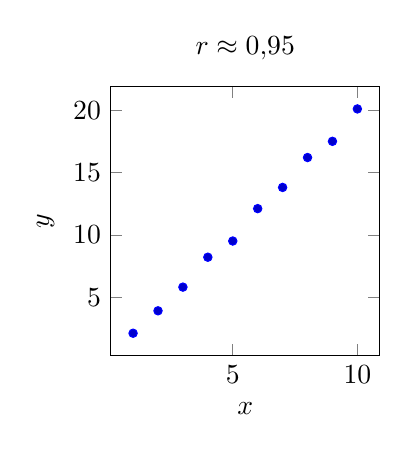
\begin{tikzpicture}
\begin{axis}[
    width=5cm, height=5cm, title={$r\approx 0{,}95$},
    xlabel=$x$, ylabel=$y$, only marks, mark size=1.5pt
]
\addplot coordinates {
(1,2.1)(2,3.9)(3,5.8)(4,8.2)(5,9.5)(6,12.1)(7,13.8)(8,16.2)(9,17.5)(10,20.1)
};
\end{axis}
\end{tikzpicture}
\hspace{1cm}
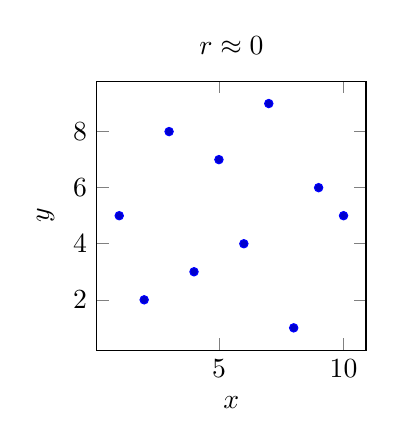
\begin{tikzpicture}
\begin{axis}[
    width=5cm, height=5cm, title={$r\approx 0$},
    xlabel=$x$, ylabel=$y$, only marks, mark size=1.5pt
]
\addplot coordinates {
(1,5)(2,2)(3,8)(4,3)(5,7)(6,4)(7,9)(8,1)(9,6)(10,5)
};
\end{axis}
\end{tikzpicture}
\hspace{1cm}
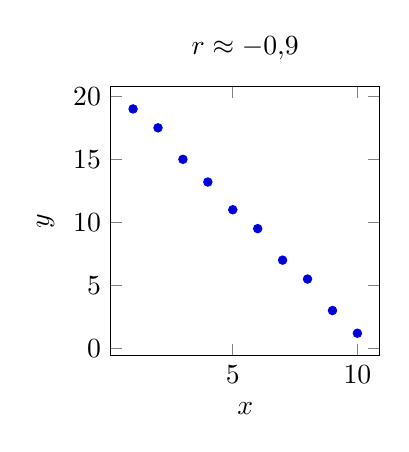
\begin{tikzpicture}
\begin{axis}[
    width=5cm, height=5cm, title={$r\approx -0{,}9$},
    xlabel=$x$, ylabel=$y$, only marks, mark size=1.5pt
]
\addplot coordinates {
(1,19)(2,17.5)(3,15)(4,13.2)(5,11)(6,9.5)(7,7)(8,5.5)(9,3)(10,1.2)
};
\end{axis}
\end{tikzpicture}
\end{center}

% ------------------------------------------------------------
\section{Impl\'ementation Python}
% ------------------------------------------------------------

\begin{python}
\begin{minted}{python}
import numpy as np
import pandas as pd
import matplotlib.pyplot as plt
from scipy import stats

# Donnees
salaires = np.array([1800, 1950, 2100, 2100, 2200, 2300, 2350, 2400,
                     2500, 2600, 2650, 2700, 2800, 2900, 3100, 3200,
                     3500, 3800, 4500, 8000])

# Mesures de tendance centrale
print(f"Moyenne    : {np.mean(salaires):.2f}")
print(f"Mediane    : {np.median(salaires):.2f}")
print(f"Mode       : {stats.mode(salaires, keepdims=True).mode[0]}")

# Mesures de dispersion
print(f"Ecart-type : {np.std(salaires, ddof=1):.2f}")
print(f"Variance   : {np.var(salaires, ddof=1):.2f}")
print(f"IQR        : {stats.iqr(salaires):.2f}")
print(f"CV         : {np.std(salaires, ddof=1)/np.mean(salaires):.4f}")

# Mesures de forme
print(f"Skewness   : {stats.skew(salaires):.4f}")
print(f"Kurtosis   : {stats.kurtosis(salaires):.4f}")  # excess kurtosis

# Visualisations
fig, axes = plt.subplots(1, 3, figsize=(14, 4))
axes[0].hist(salaires, bins=8, edgecolor='black', alpha=0.7)
axes[0].set_title("Histogramme")
axes[0].set_xlabel("Salaire (EUR)")

axes[1].boxplot(salaires, vert=True)
axes[1].set_title("Boite a moustaches")

# Fonction de repartition empirique
x_sorted = np.sort(salaires)
y_ecdf = np.arange(1, len(x_sorted)+1) / len(x_sorted)
axes[2].step(x_sorted, y_ecdf, where='post')
axes[2].set_title("ECDF")
axes[2].set_xlabel("Salaire (EUR)")
axes[2].set_ylabel("F_n(x)")

plt.tight_layout()
plt.savefig("ch01_descriptive.pdf")
plt.show()
\end{minted}
\end{python}

% ------------------------------------------------------------
\section{Exercices}
% ------------------------------------------------------------

\begin{exercice}[$\star$ -- Calculs de base]
On mesure les temp\'eratures (en ${}^\circ$C) sur 10 jours : $12, 14, 15, 13, 16, 18, 14, 15, 17, 16$.
\begin{enumerate}
\item Calculer la moyenne, la m\'ediane et le mode.
\item Calculer la variance (corrig\'ee), l'\'ecart-type et l'IQR.
\item Tracer l'histogramme et la bo\^ite \`a moustaches avec Python.
\end{enumerate}
\end{exercice}

\begin{exercice}[$\star$ -- Donn\'ees bivari\'ees]
Un cours de statistique a les notes suivantes pour le partiel (P) et l'examen final (E) de 8 \'etudiants :
\begin{center}
\begin{tabular}{ccccccccc}
\toprule
\'Etudiant & 1 & 2 & 3 & 4 & 5 & 6 & 7 & 8 \\
\midrule
P & 8 & 12 & 14 & 10 & 16 & 6 & 18 & 11 \\
E & 9 & 13 & 15 & 12 & 17 & 8 & 19 & 13 \\
\bottomrule
\end{tabular}
\end{center}
Calculer $r_{PE}$ et interpr\'eter.
\end{exercice}

\begin{exercice}[$\star\star$ -- Propri\'et\'es de la moyenne]
\begin{enumerate}
\item Montrer que $\sum_{i=1}^n (x_i - \bar{x}) = 0$.
\item Montrer que $\bar{x}$ minimise $\sum_{i=1}^n (x_i - c)^2$ sur $c\in\R$.
\item En d\'eduire que $s^2 = \frac{1}{n-1}\left(\sum x_i^2 - n\bar{x}^2\right)$.
\end{enumerate}
\end{exercice}

\begin{exercice}[$\star\star$ -- In\'egalit\'e de Tchebychev empirique]
Montrer que pour tout $k>0$, la proportion d'observations $x_i$ v\'erifiant $|x_i-\bar{x}|>ks$ est au plus $1/k^2$.
\end{exercice}

\begin{exercice}[$\star\star\star$ -- Projet : analyse exploratoire]
T\'el\'echarger un jeu de donn\'ees r\'eel (par ex.\ \texttt{tips} de \texttt{seaborn} ou un fichier CSV de l'INSEE). Produire un rapport complet : statistiques descriptives, visualisations (histogrammes, boxplots, scatter plots), identifier les valeurs aberrantes, commenter la forme de la distribution.
\end{exercice}

% ------------------------------------------------------------
\begin{formules}
\begin{align*}
\bar{x} &= \frac{1}{n}\sum_{i=1}^n x_i &
s^2 &= \frac{1}{n-1}\sum_{i=1}^n(x_i-\bar{x})^2 \\
\mathrm{IQR} &= Q_3 - Q_1 &
r_{xy} &= \frac{s_{xy}}{s_x s_y} \\
\gamma_1 &= \frac{1}{n}\sum\left(\frac{x_i-\bar{x}}{s}\right)^3 &
\gamma_2 &= \frac{1}{n}\sum\left(\frac{x_i-\bar{x}}{s}\right)^4-3 \\
\hat{F}_n(x) &= \frac{1}{n}\sum_{i=1}^n \mathbf{1}_{x_i\leq x} &
\mathrm{CV} &= s/\bar{x}
\end{align*}
\end{formules}
